\documentclass[aspectratio=169]{beamer}

\mode<presentation>
\usetheme{Boadilla}
\definecolor{redback}{RGB}{140,0,0}
\definecolor{blue}{RGB}{30,90,205}
\definecolor{red}{RGB}{213,94,0}
\definecolor{green}{RGB}{0,128,0}
\setbeamercolor{title}{fg=redback}
\setbeamercolor{frametitle}{fg=redback}
\setbeamercolor{block title}{bg=redback, fg=white}
\setbeamercolor{block body}{bg=white}
\setbeamercolor{structure}{fg=redback}
\setbeamercolor{item projected}{fg=white}
\setbeamercolor{item}{fg=redback}
\setbeamercolor{subitem}{fg=redback}
\setbeamercolor{section in toc}{fg=redback}
\setbeamercolor{description item}{fg=redback}
\setbeamercolor{caption name}{fg=redback}
\setbeamercolor{button}{bg=redback, fg=white}
\setbeamercolor{caption name}{fg=redback}
\usepackage{graphics}
\usepackage{tikz}
\usepackage{amsmath}
\usepackage{bbm}
\usetikzlibrary{decorations.pathreplacing}
\usepackage{geometry}
\usepackage{booktabs}
\usepackage{multirow, makecell}
\usepackage{float}
\usepackage{fancyvrb}
\usepackage{kotex}
\usepackage{caption}
\usepackage{subcaption}
\usepackage{adjustbox}
\usepackage{hyperref}
\usepackage{threeparttable}
\usepackage[scaled=0.92]{helvet}
\usepackage[default]{lato} %If I want a twist
\newenvironment{wideitemize}{\itemize\addtolength{\itemsep}{10pt}}{\enditemize}
\newenvironment{wideenumerate}{\enumerate\addtolength{\itemsep}{10pt}}{\endenumerate}
\newenvironment{widedescription}{\description\addtolength{\itemsep}{10pt}}{\enddescription}
\hypersetup{
colorlinks=true,
linkcolor=redback,
filecolor=green, 
urlcolor=blue,
}
\beamertemplatenavigationsymbolsempty
\setbeamercolor{author in head/foot}{bg=white, fg=redback}
\setbeamercolor{title in head/foot}{bg=white, fg=redback}
\setbeamercolor{date in head/foot}{bg=white, fg=redback}
\setbeamercolor{section in head/foot}{bg=white, fg=redback}
\setbeamercolor{page number in head/foot}{bg=white, fg=redback}
\setbeamercolor{headline}{bg=redback}
\setbeamertemplate{footline}{
    \leavevmode%
    \hbox{%
        \begin{beamercolorbox}[wd=.333333\paperwidth,ht=2.25ex,dp=1ex,center]{date in head/foot}%
            \usebeamerfont{date in head/foot}\insertshortdate
        \end{beamercolorbox}%
        \begin{beamercolorbox}[wd=.444444\paperwidth,ht=2.25ex,dp=1ex,center]{title in head/foot}%
            \usebeamerfont{title in head/foot}\insertshorttitle
        \end{beamercolorbox}%
        \begin{beamercolorbox}[wd=.222222\paperwidth,ht=2.25ex,dp=1ex,center]{page number in head/foot}%
            \usebeamerfont{page number in head/foot} \insertframenumber{} / \inserttotalframenumber
        \end{beamercolorbox}}%
        \vskip0pt%
    }

\setbeamertemplate{section in toc}[sections numbered]
\setbeamertemplate{subsection in toc}{\leavevmode\leftskip=3em\rlap{\hskip-1.75em\inserttocsectionnumber.\inserttocsubsectionnumber}\inserttocsubsection\par}
\setbeamerfont{subsection in toc}{size=\footnotesize}

\newenvironment{transitionframe}{\setbeamercolor{background canvas}{bg=redback}\setbeamertemplate{footline}{} \begin{frame}}{\end{frame}}
\newcommand{\ROM}[1]
    {\MakeUppercase{\romannumeral #1}}
    \DeclareMathOperator*{\plim}{plim}
\makeatletter
\let\@@magyar@captionfix\relax
\makeatother


\title[Recitation 9 (Intro to Econometrics \ROM{2})]{Recitation 9: Local polynomials their asymptotics} % Change this regularly
\author[]{Seung-hun Lee }
\institute[]{Columbia University \\ Introduction to Econometrics \ROM{2} Recitation}

\date[April 4th, 2022]{April 4th, 2022}

\begin{document}
\begin{frame}
\titlepage
\end{frame}


%%% Color slides for section headers: Use for colloquium version (The ones bewteen \iffals and \fi)

\begin{transitionframe}
  \begin{center}
         { \Huge \textcolor{white}{Kernel density regression}}
       \end{center}
\end{transitionframe}

\begin{frame}
\frametitle{Kernel density estimates are CAN....}
\begin{itemize}
\item Consistency: Kernel estimator achieves pointwise consistency, or consistent at particular point $y=y_0$ if both the bias and the variance disappear at that point
\begin{itemize}
\item Stronger version with uniform continuity: $\hat{f}_n(y)$ is consistent at all values of $y$ if $\hat{f}_n(y)$ uniformly converges to $f(y)$
\end{itemize}
\item Asymptotically normal: Estimator is recentered differently, but still normal
\begin{itemize}
\item We know $E[\hat{f}_n(y)]=f(y)+\frac{1}{2}h^2(f''(y))\int_{-\infty}^\infty u^2K(u)du$ and $Var(\hat{f}_n(y)) = \frac{1}{nh}f(y) \int_{-\infty}^\infty K^2(u)du$
\item Thus the CLT leads to
\[
\sqrt{nh}\left(\hat{f}_n(y) - f(y) - \frac{1}{2}h^2(f''(y))\int_{-\infty}^\infty u^2K(u)du\right)\sim N\left(0, f(y) \int_{-\infty}^\infty K^2(u)du\right)
\]
\end{itemize}
\end{itemize}
\end{frame}

\begin{frame}
\frametitle{...Just not in a typical manner}
\[
\sqrt{\color{red}{nh}}\left(\hat{f}_n(y) - f(y) \color{blue}{- \frac{1}{2}h^2(f''(y))\int_{-\infty}^\infty u^2K(u)du} \color{black} \right)\sim N\left(0, f(y) \int_{-\infty}^\infty K^2(u)du\right)
\]
\begin{itemize}
\item Effective sample is $\color{red}{nh}$: If $h$ is optimally chosen, effective sample size is  $O(n^{4/5})$
\item $\color{blue}{\frac{1}{2}h^2(f''(y))\int_{-\infty}^\infty u^2K(u)du}$: Cannot ignore them since bias and standard errors move at same rate (parametrics: bias converged to 0 quicker)
\item Further conditions (not as significant as the two above): $f$ is twice continuously differentiable and $\int_{-\infty}^\infty u^2K(u)du$ is constant to pin the value of bias
\end{itemize}
\end{frame}

\begin{frame}
\frametitle{Confidence intervals are centered with bias correction!}
\begin{itemize}
\item We define a 95\% pointwise confidence interval at particular $y$ value as
\small{\[
CI = \left[\hat{f}_n(y)-b(y)-1.96\sqrt{\frac{1}{nh}\hat{f}_n(y) \int_{-\infty}^\infty K^2(u)du},\ \hat{f}_n(y)-b(y)+1.96\sqrt{\frac{1}{nh}\hat{f}_n(y) \int_{-\infty}^\infty K^2(u)du}\right]
\]}\normalsize
where $b(y)=\hat{f}_n(y)-\frac{1}{2}h^2(f''(y))\int_{-\infty}^\infty u^2K(u)du$
\item The problem is also complicated further due to the existence of $f''(y)$
\item Alternative: Confidence bands are computed for $f(y)$ over all possible values of $y$, which results in a wider confidence intervals than the pointwise ones
\end{itemize}
\end{frame}

\begin{frame}
\frametitle{One dimensional kernel was already hard. How about a multiple?}
\begin{itemize}
\item  Now assume that $y$ is not necessarily a scalar, but of dimension $d$. 
\item Then we can use a $d$-dimensional kernel $K$ and estimate $f(y)$ with
 \[
 \hat{f}_n(y)= \frac{1}{nh^d}\sum_{i=1}^nK\left(\frac{y-y_i}{h}\right)
 \]
 where $K$ can be a $d$-product of a uni-dimensional kernels.
 \item  We are not necessarily confined to using a same bandwith for all $d$ kernels 
 \begin{itemize}
 \item If variance of $y_1$ is larger than $y_2$ you may want higher $h_1$ relative to $h_2$
 \item Sphericize them if necessary if you suspect correlation between kernels (like GLS)
 \end{itemize}
 \item But this is only a minor problem: Optimal bandwidth is even more complicated
\end{itemize}
\end{frame}

\begin{frame}
\frametitle{Optimal bandwidth: Solving again for AMISE }
\begin{itemize}
\item Curse of dimensionality has to do with bandwidth costs
\item Variance has a different leading term (leading term)
 \footnotesize{\begin{align*}
 E[\hat{f}_n(y)^2]&=E\left[\frac{1}{n^2h^{2d}}\left(\sum_{i=1}^nK\left(\frac{y-y_i}{h}\right)\right)^2\right]\\
 &=E\left[\frac{1}{n^2h^{2d}}\left(\sum_{i=1}^nK^2\left(\frac{y-y_i}{h}\right)+2\sum_{i<j} K\left(\frac{y-y_i}{h}\right)K\left(\frac{y-y_j}{h}\right)\right)\right]\\
 &=\frac{1}{nh^{2d}}\int_{-\infty}^\infty K^2\left(\frac{y-t}{h}\right)f(t)dt+\frac{n(n-1)}{n^2h^{2d}}\left(\int_{-\infty}^\infty K\left(\frac{y-t}{h}\right)f(t)dt\right)^2
 \end{align*}}\normalsize
\item The leading term is $\frac{1}{nh^{2d}}\int_{-\infty}^\infty K^2\left(\frac{y-t}{h}\right)f(t)dt \simeq \frac{1}{nh^d}\int K^2(-u)f(y)du$ since $u$ is actually $d$-dimensional. 
\item Thus, the variance is now $O\left(\frac{1}{nh^d}\right)$. 
\end{itemize}
\end{frame}

\begin{frame}
\frametitle{Optimal bandwidth now leads to even slower convergence}
\begin{itemize}
\item Bias is at the same rate
\footnotesize{ \begin{align*}
  E[\hat{f}_n(y)]&=E\left[ \frac{1}{nh^d}\sum_{i=1}^nK\left(\frac{y-y_i}{h}\right) \right]\\
  &=\frac{1}{h^d}\int_{-\infty}^\infty K\left(\frac{y-t}{h}\right)f(t)dt\\
    &=\int_{-\infty}^\infty K(-u)f(y+uh)du \ (\because\text{$u=\frac{t-y}{h}$ and $K(\cdot)$ is an $d$-dimensional multi-kernel})
 \end{align*}}\normalsize
 apply same procedure as the univariate kernel to get bias$= \frac{1}{2}\int_{-\infty}^\infty K(u)h^2u^2f''(y)du$
\item   What this means is that $AMISE=Ah^4+\frac{B}{nh^d}$ and the optimal $h$ is solved as
 \[
 h=\left(\frac{Bd}{4An}\right)^{1/(4+d)}
 \]
 \item  $h$ will be in $n^{-\frac{1}{4+d}}$, bias and standard errors are in $n^{-\frac{2}{4+d}}$ (even slower!)
\end{itemize}
\end{frame}

\begin{frame}
\frametitle{What does it all mean? LARGE observations are needed}
\begin{itemize}
\item Larger observations needed to achieve similar precisions as in lower-level kernel density estimation
\item Rigorously, the sparseness problem becomes bigger with larger dimensions - fewer observations around $y$ receive substantial weight (or an empty space phenomenon)
\item  Silverman documents that the required sample size to accurately estimate density of a standard normal at $0$ rises drastically - 4 for univariate to 842,000 in 10-dimensional
\end{itemize}
\end{frame}


\begin{transitionframe}
  \begin{center}
         { \Huge \textcolor{white}{Local polynomial regression}}
       \end{center}
\end{transitionframe}

\begin{frame}
\frametitle{Conditional expectations from nonparametric approach is possible}
\begin{itemize}
\item Given $(y_i,x_i)$, we are attempting to capture $E[g(y,x)|x]=m(x)$ for some $g(y,x)$
\item Frequently, we let $g(y,x)=y$
\item Conditional expectation is written as 
 \begin{align*}
 E[y|x]&=\int y f_{Y|X}(y|x)dy \\
 &=\int y \frac{f_{Y,X}(y,x)}{f_{X}(x)}dy \ (\because \text{Relation between conditional, marginal, and joint pdf})\\
 &=\frac{\int yf_{Y,X}(y,x)dy}{\int f_{Y,X}(y,x)dy} \ (\because f_X(x) = \int f_{Y,X}(y,x)dy)
 \end{align*}
 \item Key? Replace $f_{Y,X}$ with its kernel estimator (For easy life, let both be a scalar)
\end{itemize}
\end{frame}

\begin{frame}
\frametitle{Numerator to a kernel density estimate}
\begin{itemize}
\item Numerator
\begin{align*}
 \int y \hat{f}(y,x)dy&=\int y \frac{1}{nh^2}\sum_{i=1}^n K\left(\frac{x-x_i}{h}\right)K\left(\frac{y-y_i}{h}\right)dy\\
 &= \frac{1}{nh^2}\sum_{i=1}^n K\left(\frac{x-x_i}{h}\right)\int yK\left(\frac{y-y_i}{h}\right)dy\\
 &=\frac{1}{nh^2}\sum_{i=1}^n K\left(\frac{x-x_i}{h}\right)\int (y_i+sh)K\left(s\right)hds \ \left(\because s=\frac{y-y_i}{h}\right)\\
 &= \frac{1}{nh}\sum_{i=1}^n K\left(\frac{x-x_i}{h}\right)y_i\ (\because \int K(s)ds=1, \int sK(s)ds=0)
 \end{align*}
\end{itemize}
\end{frame}

\begin{frame}
\frametitle{Denominator and the complete set}
\begin{itemize}
\item Denominator
\[
 \begin{aligned}
 \int \hat{f}_{Y,X}(y,x)dy&=\int \frac{1}{nh^2}\sum_{i=1}^nK\left(\frac{x-x_i}{h}\right)K\left(\frac{y-y_i}{h}\right)dy\\
 &=\frac{1}{nh^2}\sum_{i=1}^nK\left(\frac{x-x_i}{h}\right)\int K\left(\frac{y-y_i}{h}\right)dy\\
  &=\frac{1}{nh^2}\sum_{i=1}^nK\left(\frac{x-x_i}{h}\right)\int K\left(s\right)hds=\frac{1}{nh}\sum_{i=1}^nK\left(\frac{x-x_i}{h}\right) \\
\end{aligned}
\]
\item  Thus, the estimator for the conditional expectation becomes
 \[
\hat{m}(x)= \frac{\sum_{i=1}^n y_iK\left(\frac{x-x_i}{h}\right)}{\sum_{i=1}^n K\left(\frac{x-x_i}{h}\right)}
 \]
\end{itemize}
\end{frame}

\begin{frame}
\frametitle{So what is $\hat{m}(x)$ exactly?}
 \[
\hat{m}(x)= \frac{\sum_{i=1}^n y_iK\left(\frac{x-x_i}{h}\right)}{\sum_{i=1}^n K\left(\frac{x-x_i}{h}\right)}
 \]
\begin{itemize}
\item  Effectively we are putting weight $\frac{K\left(\frac{x-x_i}{h}\right)}{\sum_{i=1}^nK\left(\frac{x-x_i}{h}\right)}$ on each observation $y_i$. 
\item This is called a \textbf{local constant estimation} or \textbf{Nadaraya-Watson estimator}: When we assume $y_i = a+e_i$ for some constant $a$, weigh each observation by its kernel density $K\left(\frac{x-x_i}{h}\right)$ and solve the following minimization problem
 \[
 \hat{f}(x)=\arg\min_a\frac{1}{nh}\sum_{i=1}^n(y_i-a)^2K\left(\frac{x-x_i}{h}\right)
 \]
 The first order condition on $a$ yields the following results
 \[
 \sum_{i=1}^ny_iK\left(\frac{x-x_i}{h}\right)=a\sum_{i=1}^nK\left(\frac{x-x_i}{h}\right) \implies a= \frac{\sum_{i=1}^n y_iK\left(\frac{x-x_i}{h}\right)}{\sum_{i=1}^n K\left(\frac{x-x_i}{h}\right)}
 \]
\end{itemize}
\end{frame}

\begin{frame}
\frametitle{Asymptotics of the NW estimator: Building blocks}
 \begin{itemize}
 \item Note that  $y_i = m(x_i)+e_i = m(x) + (m(x_i)-m(x))+e_i$
\item Assume $m(x_i)=E[y|x_i]$ is twice continuously differentiable, $f(x)$ is a pdf that is once continuously differentiable, and $E[e_i|x_i]=0, E[e_i^2|x_i=x]=\sigma^2(x)<\infty$
\item  We can express the numerator of $\hat{m}(x)$ as 
\[\begin{aligned}
\frac{1}{nh}\sum_{i=1}^n y_iK\left(\frac{x-x_i}{h}\right) &=\frac{1}{nh}\sum_{i=1}^n K\left(\frac{x-x_i}{h}\right) (m(x) + (m(x_i)-m(x) )+ e_i)\\ 
&=\hat{f}(x)m(x) + \hat{m}_1(x)+\hat{m}_2(x)
\end{aligned}\]
\item $\hat{m}(x)=\frac{\hat{f}(x)m(x) + \hat{m}_1(x)+\hat{m}_2(x)}{\hat f(x)}= m(x)+\frac{\hat{m}_1(x)}{\hat{f}(x)}+\frac{\hat{m}_2(x)}{\hat{f}(x)}$
\end{itemize}
\end{frame}

\begin{frame}
\frametitle{Asymptotics bias of the NW estimator}
 \begin{itemize}
 \item We need to know $E[\hat{m}_1(x)]$ and  $E[\hat{m}_2(x)]$
 \item Since $E[e_i|x_i]=0$, then $E\left[e_iK\left(\frac{x-x_i}{h}\right) \right]=0$ and $E[\hat{m}_2(x)]=0$
\item  For $E[\hat{m}_1(x)]$, we work with
\footnotesize{\[\begin{aligned}
E[\hat{m}_1(x)]&=E\left[ \frac{1}{nh}\sum_{i=1}^n K\left(\frac{x_i-x}{h}\right) (m(x_i)-m(x))\right] = \frac{1}{h}\int K\left(\frac{s-x}{h}\right) (m(s)-m(x))f(s)ds \\
&= \int K\left(u\right) (m(x+hu)-m(x))f(x+hu)du \ \left(\because u=\frac{s-x}{h}\right)\\
&= \int K\left(u\right) (uh m'(x)+ \frac{1}{2}u^2h^2 m''(x)) (f(x)+uhf'(x))du \ \left(\because \text{two Taylor expansions!}\right)\\
&=\int h^2m'(x)f'(x) u^2 K\left(u\right)du +\int \frac{h^2}{2} m''(x)f(x) u^2K(u)du + .... \\
\end{aligned}\]}\normalsize
\item ... includes higher order terms than $h^2$
 \end{itemize}
\end{frame}

\begin{frame}
\frametitle{Asymptotics bias has complexities with $m$ and $f$ functions}
 \begin{itemize}

\item  If we have $\hat{f}(x)$ that is a consistent density estimator for $f(x)$, we can now write
\[
E[\hat{m}(x)]=m(x) + \int h^2\frac{m'(x)f'(x)}{f(x)} u^2 K\left(u\right)du +\int \frac{h^2}{2} m''(x)u^2K(u)du
\]
\item Therefore, the bias is still of order $h^2$, but the exact expression becomes
\[
E[\hat{m}(x)]-m(x) = h^2 \left( \frac{m'(x)f'(x)}{f(x)} + \frac{m''(x)}{2} \right)\int u^2K(u)du
\]
 \end{itemize}
\end{frame}

\begin{frame}
\frametitle{Asymptotics variance of the NW estimator}
 \begin{itemize}

\item  We have
\footnotesize{\[\begin{aligned}
var(\hat{m}_2(x))&=E\left[\left(\frac{1}{nh}\sum_{i=1}^n K\left(\frac{x_i-x}{h}\right)e_i \right)^2\right]=\frac{1}{nh^2}E\left[\left(K\left(\frac{x_i-x}{h}\right)e_i \right)^2\right] \ (\because IID)\\
&=\frac{1}{nh^2}E\left[\left(K\left(\frac{x_i-x}{h}\right)\sigma(x_i) \right)^2\right] \ (\because \text{condition on }x)=\frac{1}{nh^2}\int K\left(\frac{s-x}{h}\right)^2\sigma^2(s)f(s)ds \\
&=\frac{1}{nh}\int K\left(u\right)^2\sigma^2(x+hu)f(x+hu)du \simeq\frac{1}{nh}\int K\left(u\right)^2\sigma^2(x)f(x)du
\end{aligned}\]}\normalsize
\item  $var(\hat{m}_1(x))$, it is actually $O\left(\frac{h^2}{nh}\right)$ a smaller order than $O\left(\frac{1}{nh}\right)$
\item  Thus, variance is
\[
\frac{1}{nh}\int K\left(u\right)^2\sigma^2(x)f(x)du / f^2(x) = \frac{1}{nh}\frac{\sigma^2(x)}{f(x)}\int K\left(u\right)^2du 
\]
 \end{itemize}
\end{frame}

\begin{frame}
\frametitle{Asymptotic distribution of NW}
 \begin{itemize}
\item As a result, the asymptotic distribution of the local constant estimator is
\footnotesize{\[
\sqrt{nh}\left(\hat{m}(x)-m(x)-h^2 \left( \color{red}{\frac{m'(x)f'(x)}{f(x)}} \color{black}+ \frac{m''(x)}{2} \right)\int u^2K(u)du\right)\sim N\left(0, \frac{\sigma^2(x)}{f(x)}\int K\left(u\right)^2du \right)
\]}\normalsize
\item NW estimators become inaccurate as $f(x)$ is small or at the boundary value
\item Moreover, the estimate also becomes volatile with $\sigma^2(x)$ - the variance of the $Y$ conditional on $X$
\item Bandwidth choice is tougher
 \end{itemize}
\end{frame}

\begin{frame}
\frametitle{Something better: Local linear estimation}
 \begin{itemize}
\item   In mathematical expression, we solve
 \[
 \min_{a,b}\frac{1}{nh}\sum_{i=1}^n(Y_i-a-b(x-x_i))^2K\left(\frac{x-x_i}{h}\right)
 \]
 and obtain that $\hat{a}=\hat{g}$ and $\hat{b}$ is an estimate of $\frac{\partial g(x)}{\partial x}$
 \item Lesser bias if true DGP is linear and better performance at the boundary
 \item Easier expression for asymptotics: We have explicitly modeled the linear term by controlling for $x-x_i$, and coefficient on this will estimate $m'(x)$. ($ y_i = m(x_i)+e_i \simeq m(x) + m'(x)(x_i-x)+e_i$)
 \item The end result for the asymptotic distribution of local linear estimator is 
 \[
 \sqrt{nh}\left(\hat{m}(x)-m(x)-h^2 \frac{m''(x)}{2} \int u^2K(u)du\right)\sim N\left(0, \frac{\sigma^2(x)}{f(x)}\int K\left(u\right)^2du \right)
 \]
 \end{itemize}
\end{frame}


\begin{frame}
\frametitle{Seminonparametric regressions}
 \begin{itemize}
\item Idea:  If we are sure that $f(y)$ can be characterized by $f_{m,\sigma}$, we can choose a family of positive functions $P_\theta^1, P_\theta^2,...(\because \text{Weierstrass approximation thm})$ and maximize over
\[
\sum_{i=1}^n \log{f_{m,\sigma}(y_i)}P_\theta^M(y_i)
\]
\begin{itemize}
\item Mixture of normals is a special case
 \end{itemize}
\item Series estimation:  Run a linear regression $ y_i = \sum_{k=1}^MP_k(x_i)\theta_k+\epsilon_i$, 
where $P_k$ is an orthonormal basis and the $\sum_{k=1}^MP_k(x_i)\theta_k$ part is a series approximation to $g(x)$
\item Sieve estimation: Similar to series estimation, where the choice of the basis is data-dependent (Splines or polygonals)
 \end{itemize}
\end{frame}

\begin{frame}
\frametitle{Black et al 2019 Restud: Linearity between parental and child wealth}
 \begin{itemize}
\item Relationship of intergenerational wealth correlation is linear, with stronger role by the adoptive parents than biological
\begin{figure}[H]
\centering
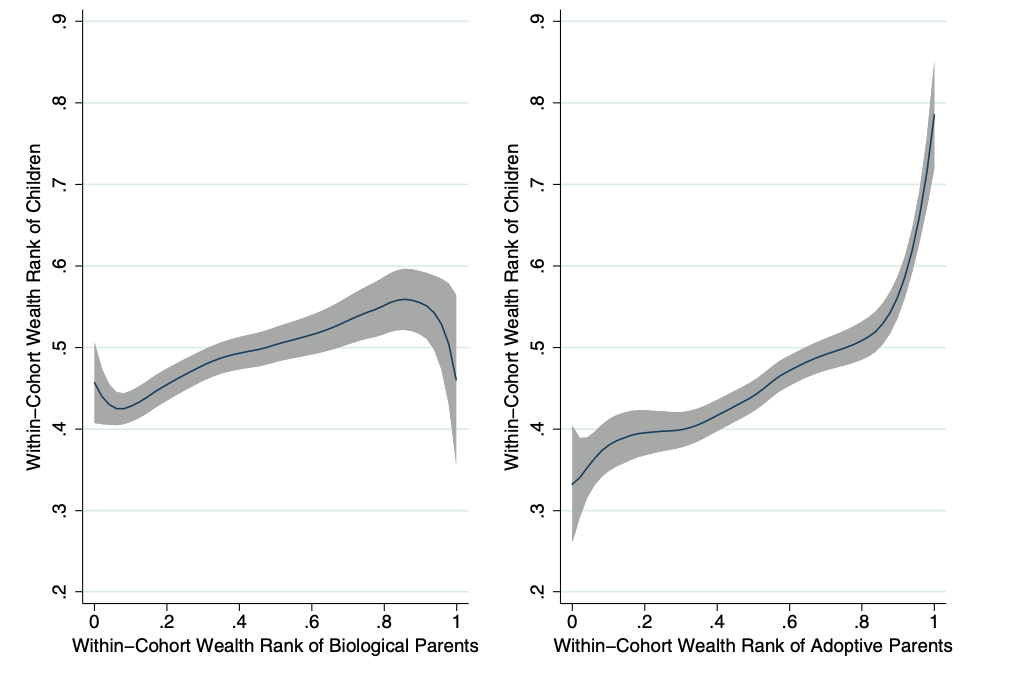
\includegraphics[keepaspectratio, width=0.6\textwidth]{black2.png}
\end{figure}
 \end{itemize}
\end{frame}

\begin{frame}
\frametitle{Brückner, Ciccone ECMA 2011: Rainfall, income, and democracy}
 \begin{itemize}
\item Rainfall shock is positively correlated with income and is followed by an improvement in institutions
\begin{itemize}
\item Negative rainfall shocks (drought) $\to$ drop in income $\to$ protests and institutional change
\end{itemize}
\begin{figure}[H]
\centering
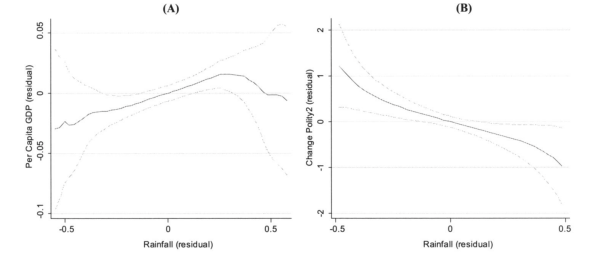
\includegraphics[keepaspectratio, width=0.8\textwidth]{bc_etca.png}
\end{figure}
 \end{itemize}
\end{frame}
%%%%%%%%%%%
\end{document}
